\section{Results} 
To make the simulation easy to understand we started with the baseline model with two covariates that was split into the different model sets. We then started adding the different flexibilities one at a time to see how much each flexibility by itself would contribute to the FPP and FPR compared to the baseline model.

\subsection{Worst-case scenario}
Under different conditions, the FPP was as high as 99\%. There were several ways to obtain a result like this. In general, the covariates needed to be binary and dummy coded and interactions used without including main effects. In such case, a 99\% FPP could be obtained with only two covariates and a big enough sample (see Figure 4). Alternatively, a 99\% FPP could also be obtained using a smaller sample and more than two covariates (see Figure 3). In the same sets, the FPR was as high as 35\%. In other words, in the sets where there was a 99\% chance to find a significant result, around 35\% of the models had either a significant main effect or interaction effect with the variable of interest. 

\subsection{Effect of model specification}
The FPP and FPR for the different model sets can be found in Figure 1. Looking at the FPP and FPR between the different sets, it is clear that the highest FPP and FPR could be obtained in the HCI and ME + HCI sets. This was the case both when main effects were present or not when using interactions. When main effects were not present, and covariates and the variable of interest were binary and dummy coded, the high FPP and FPR occurred because the interaction would capture the true effect from the covariates as the dummy coded variable of interest would just split the effect into the interaction and the constant. In this case, the FPP for for the HCI set was 83.4\% and 86.9\% for the ME + HCI set (sample size = 200). When the variables were continuous and everything else was equal, the FPP for the two sets was 18.9\% and 24.3\%, respectively. When we implemented the restriction that main effects should follow interactions, out of the two previously mentioned sets, only the ME + HCI set remained because the HCI set became an empty set. Here, the FPP was 20.6\% for binary variables and 18.6\% for continuous variables. Across all sets, the FPP  was 87.2\% when using two binary variables, and 24.7\% when the variables were continuous and when we had no restrictions regarding main effects, whereas the FPP was 22\% and 18.5\%, respectively, when we had such a restriction.\\ 
Not only was the FPP higher than 5\%, but the FPR was also higher in some sets (see red bars in Figure 1). In general, the proportion of models with a significant effect was around the expected 5\%, but in the sets where there were interactions between the variable of interest and covariates and main effects were not present (left hand side of Figure 1), the FPR was above 5\%. The percent of models with a significant variable of interest or interaction with the variable of interest was 31.9\% for the ME + HCI set when main effects were not included and binary data was used. Overall, the model sets where HCI was included had a higher number of models with a significant effect. \\
Adding one more covariate to the analysis (such that the analysis included three) just increased the FPP across all model sets, where it was still possible to get a higher FPP. This added effect of using one more covariate can be seen in Figure 2. The increase was the highest for the binary data and where there was no restriction that main effects should follow interactions. Several of the sets here (e.g., sets that contained HCI) had the rate of FPP just below a 100\%. This increase was also evident when we restricted the sets such that main effects should always be present when having interactions. In that case, the FPP increased by 14.3\% for the ME + HCI + CCI set with the binary variable of interest and covariates and by 13.1\% when these were continuous. The rates of FPR also increased. This increase, however, only applies for the sets where there were interactions between the variable of interest and covariates. Even though there was a higher increase when there was no restriction that main effects should be present when having interactions, we observed an increase even when the restriction was in place. Using three covariates increased the FPR for the ME + HCI + CCI set for around 3\% compared to using two covariates for both binary and continuous data. 

% plot of main analysis
\begin{figure}[hbt!]
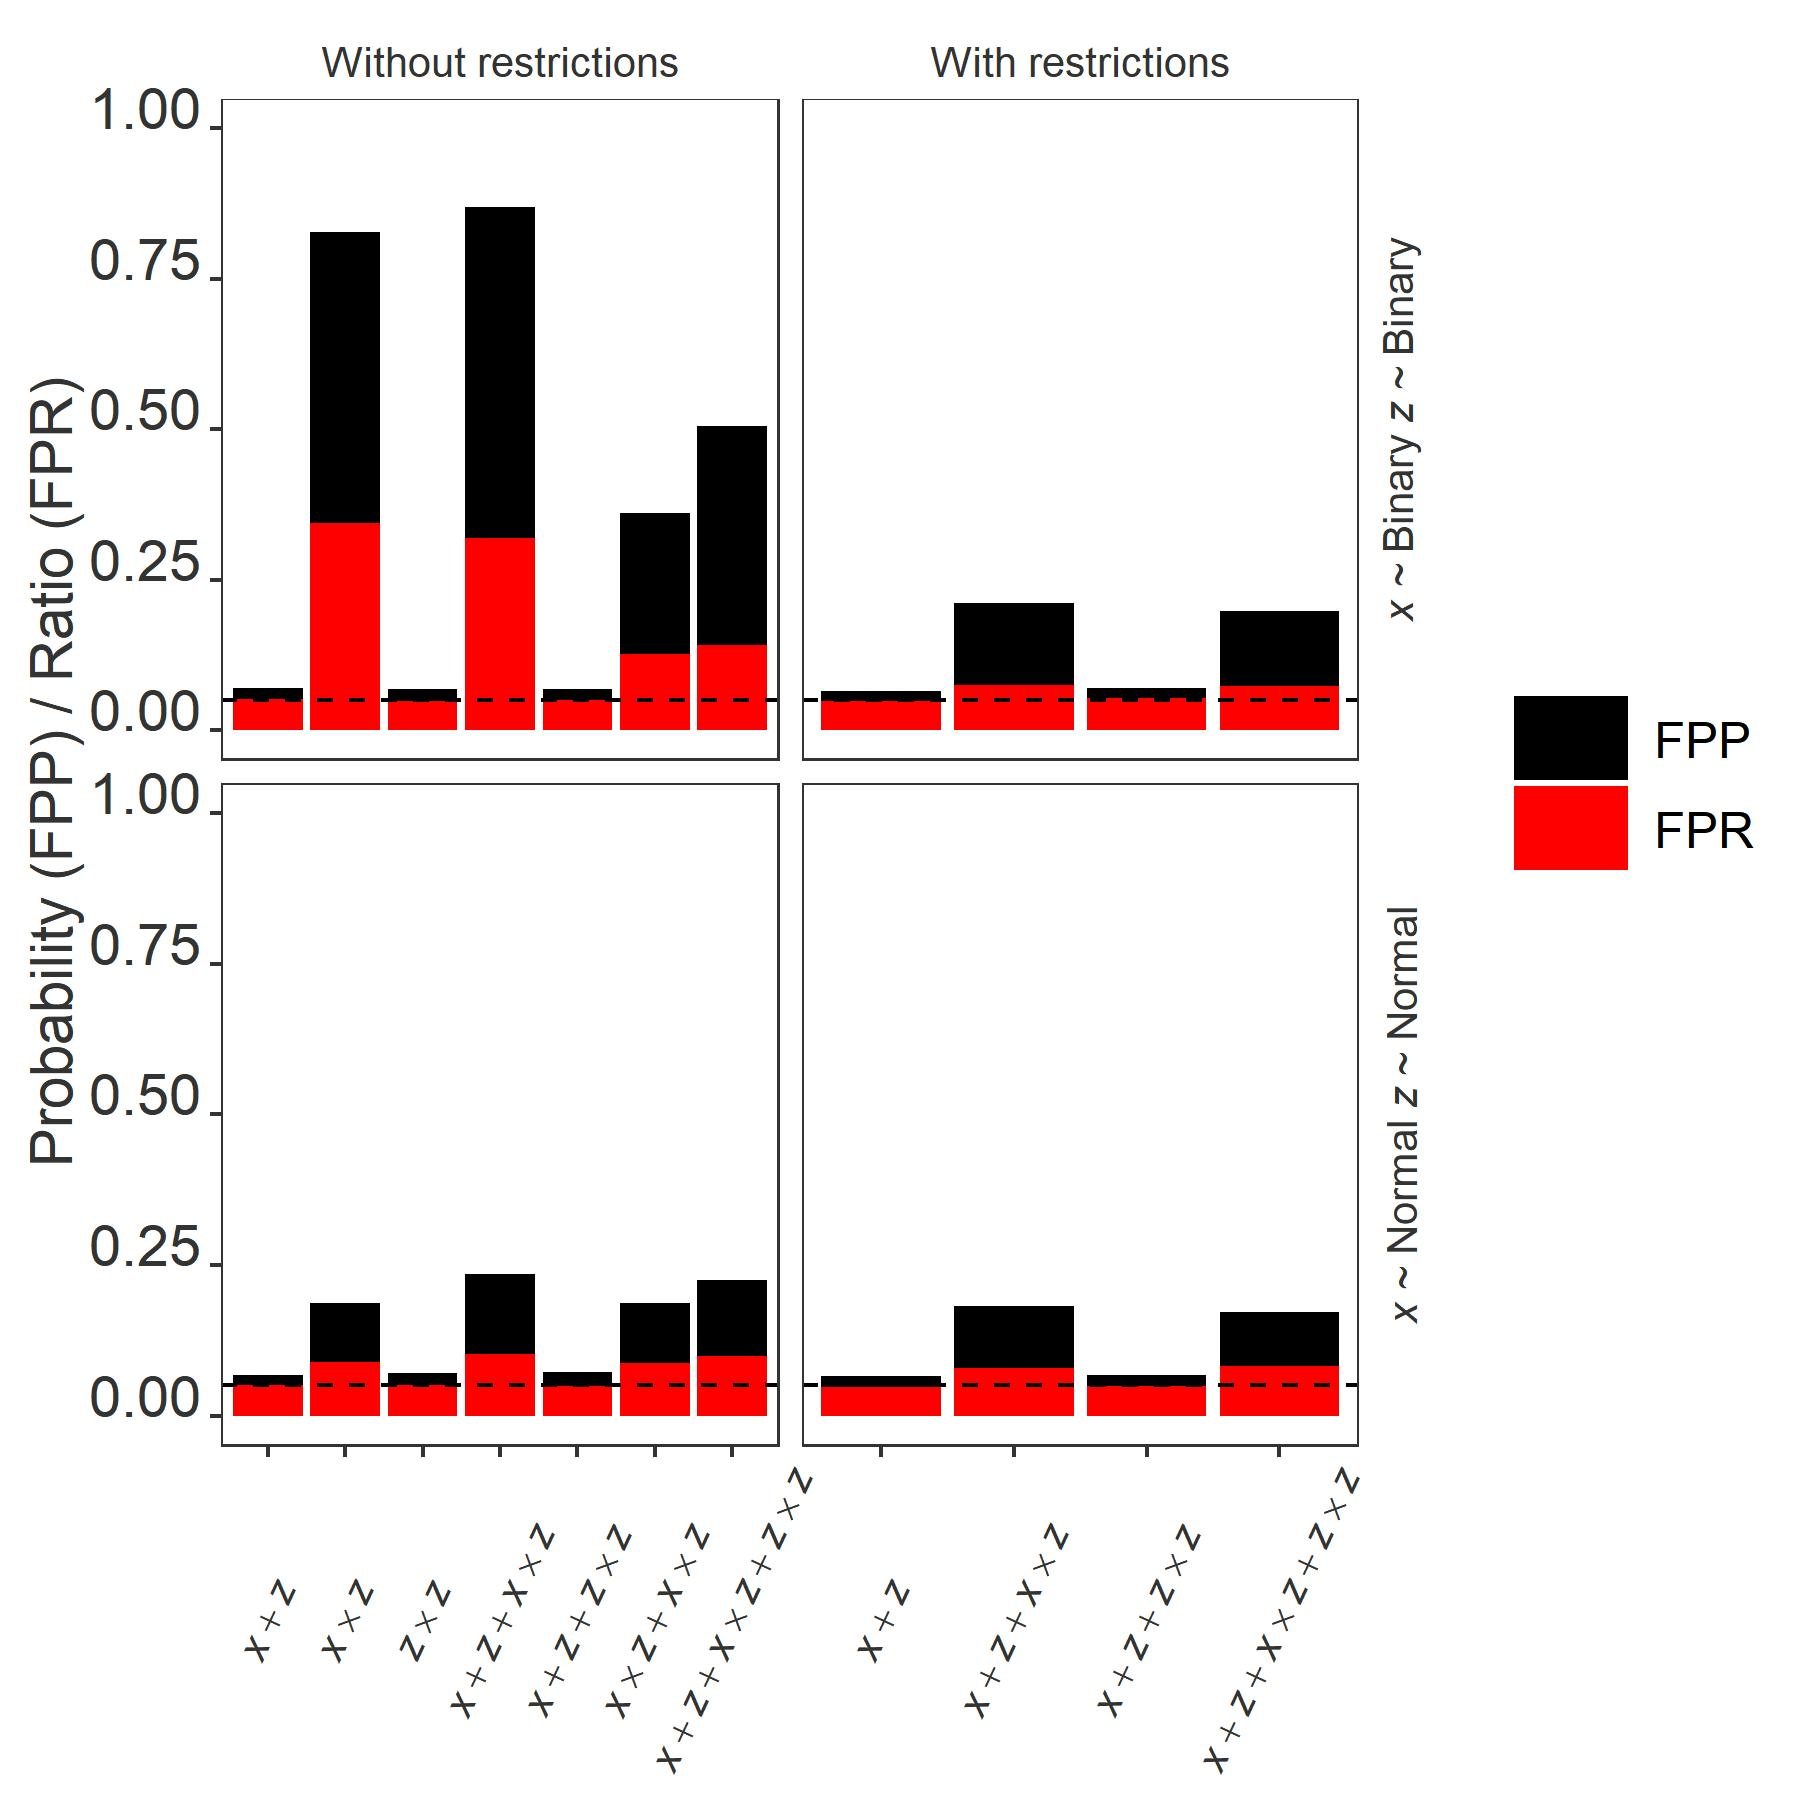
\includegraphics[width=0.6\textwidth]{R/Analysis/Result/Figures/Figure1A.jpeg}
\centering
\caption{The rates of the false-positive probability and false-positive ratio given different model sets, the presence of main effects when having interactions, and different distributions of the variable of interest and covariates. Sample size was set to 200, a correlation between the dependent variable and covariates was \textit{r}=0.2 and we used two covariates. The false-positive probability is shown in black and the false-positive ratio in red.}
\label{fig:mainfigure}
\end{figure}

% plot of main analysis
\begin{figure}[hbt!]
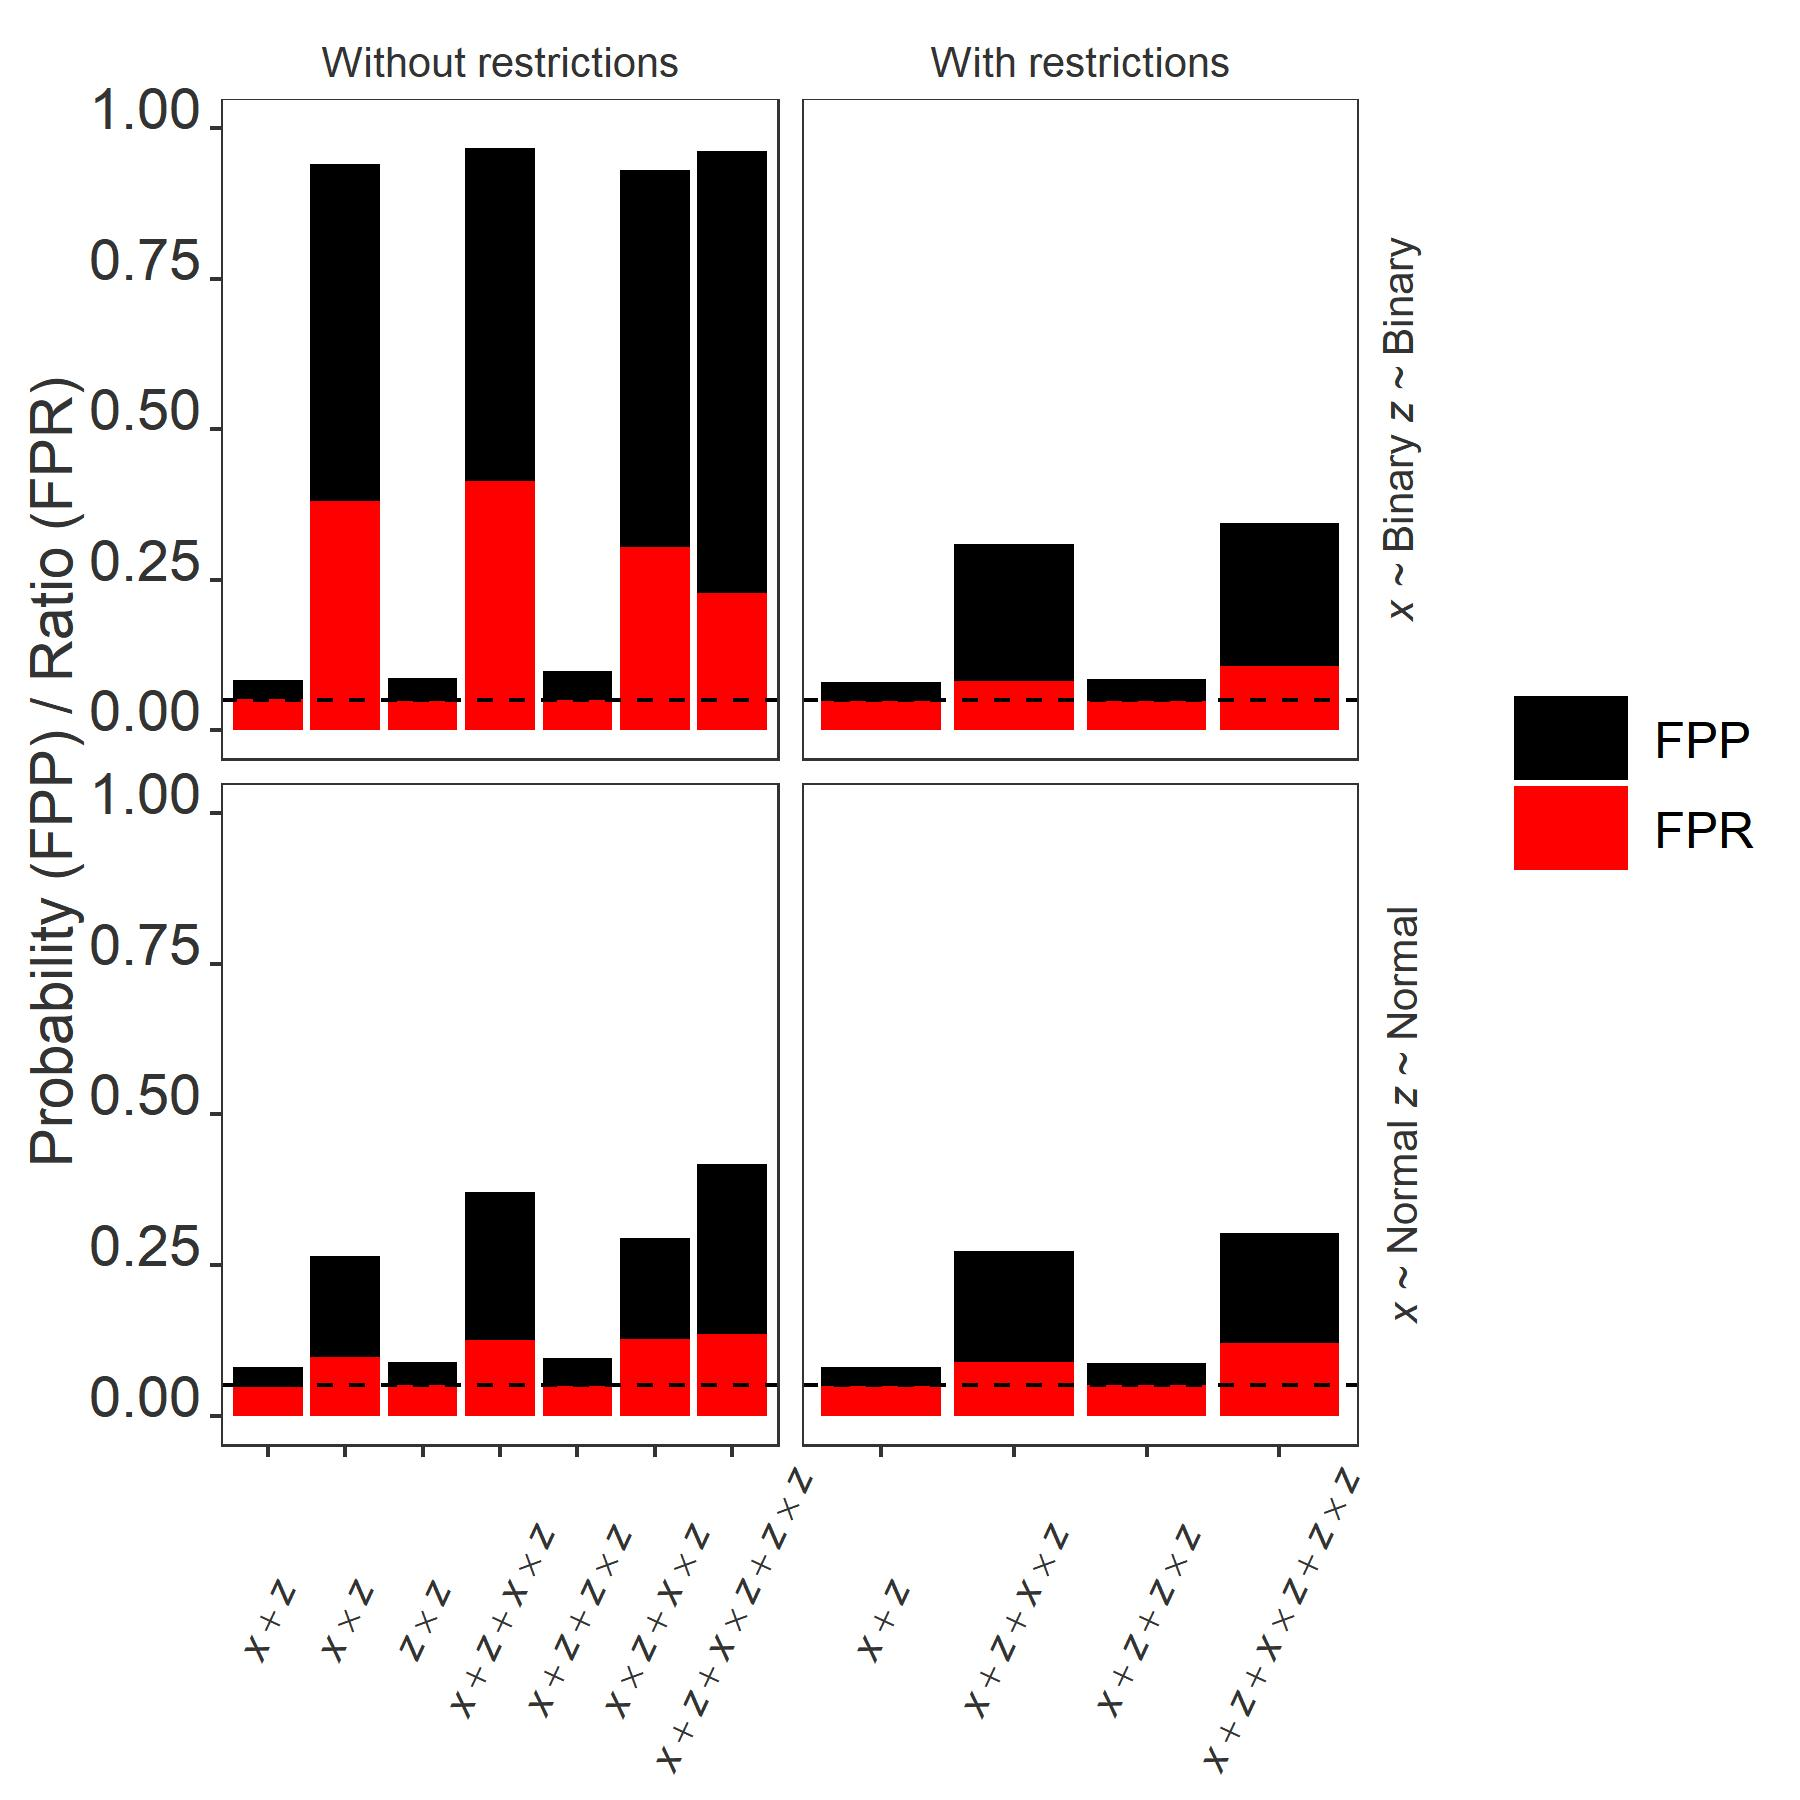
\includegraphics[width=0.6\textwidth]{R/Analysis/Result/Figures/Figure1C.jpeg}
\centering
\caption{Difference in the false-positive probability and false-positive ratio compared to the base model in Figure 1 when using one more covariate (three in total). Black bars are the added effect to the false-positive probability and red denotes the added effect to the false-positive ratio. The description of the figure is otherwise the same as for Figure 1.}
\label{fig:mainfigure}
\end{figure}

\subsection{Outlier criteria}
Here we were interested in how outlier deletion affected the FPP and FPR across the different model sets. Therefore, we computed the added effect of using the four different outlier criteria compared to not using any such criteria. Again, the sample was set to 200, and all binary variables where dummy coded. Figure 3 shows the added effect of using the outlier criteria. It can be seen that outlier deletion had a different added effect on the different model sets and data structures. We observed the biggest effect within the sets including interactions between the variable of interest and covariates. Overall, the added effect to the FPP was between 4\% and 19.4\% for the model sets where there was still room for an added effect. The lower added effects seen in some cases came from the fact that the FPP was already close to 100\%. This was the case for the sets where the variables were binary, where there was an interaction between the variable of interest and covariates, and where we allowed for models with no main effects when having interactions. On the other hand, using outlier criteria did not increase the FPR and in some cases even decreased it. 

\begin{figure}[hbt!]
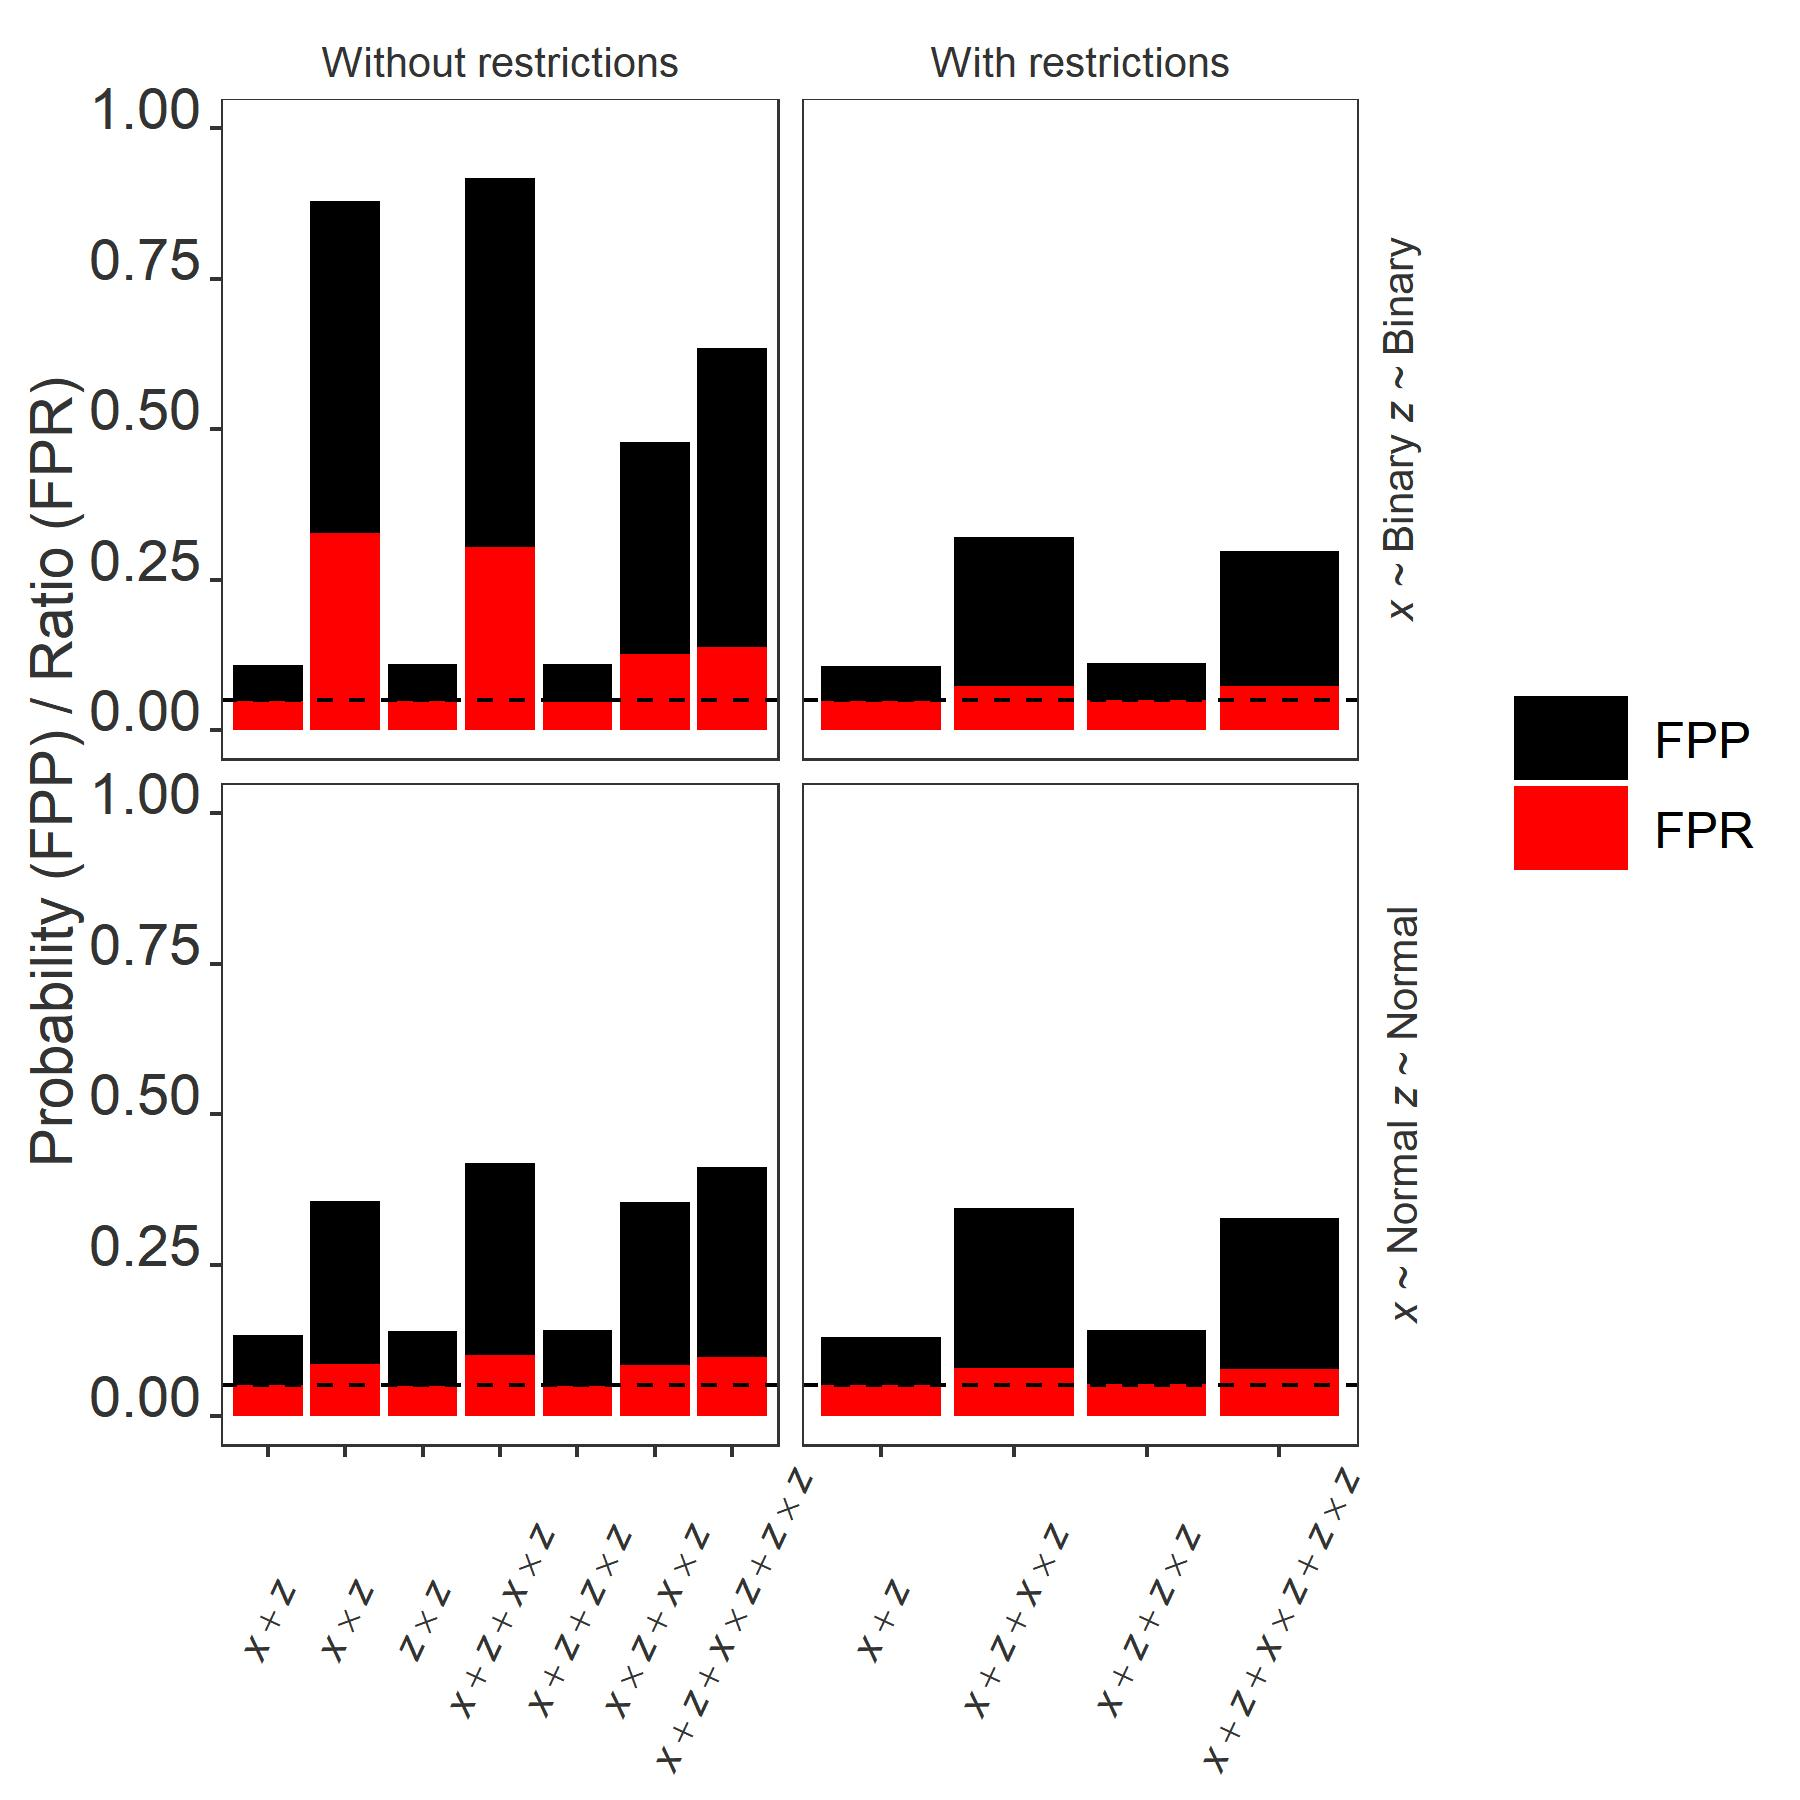
\includegraphics[width=0.6\textwidth]{R/Analysis/Result/Figures/Figure1B.jpeg}
\centering
\caption{Difference in false-positive probability and false-positive ratio compared to the base model in Figure 1 when using multiple outlier criteria. Black denotes the added effect to the false-positive probability and red denotes the added effect to the false-positive ratio.  The description of the figure is otherwise the same as for Figure 1.}
\label{fig:mainfigure}
\end{figure}

\subsection{Multiple dependent variables}
Here we looked at the effect of having multiple dependent variables on the FPP and FPR across different model sets. We did not specify any outlier criteria and all binary variables were dummy coded. Collecting multiple dependent variables and using their average increased the FPP. This was a general result regardless of data structures, model sets, and whether main effects were included or not when having interactions. The effect of using two dependent variables and their average can be seen in Figure S3 in the Supplementary Material. This increase was the highest for the sets where there were interactions between the variable of interest and covariates. For these sets, the increase in the FPP was around 15\%. The increase in the FPR seemed to be mainly driven by the increase in the number of models, as the FPR did not increase for any of the sets. 

\subsection{Sample size}
Increasing the sample size and thereby the precision of the estimates did not seem to lower the FPP. Even worse, when main effects were not included, the larger sample size increased the FPP when having interactions between the variable of interest and covariates and when these were binary (See Figure 4). In this case, the FPP went just under 100\% as the sample size increased to 300. The larger sample did not only increase the FPP, but also the FPR. The FPR got as high as 42\% for the HCI set with binary data and no main-effects-related restrictions. For continues variables, the results looked the same regardless of main effects following interactions or not, but there was still no decrease in the FPP and FPR when increasing the sample size (i.e., the FPP and FPR remained roughly constant around ... and ... respectively as the sample size increased). 


\begin{figure}[hbt!]
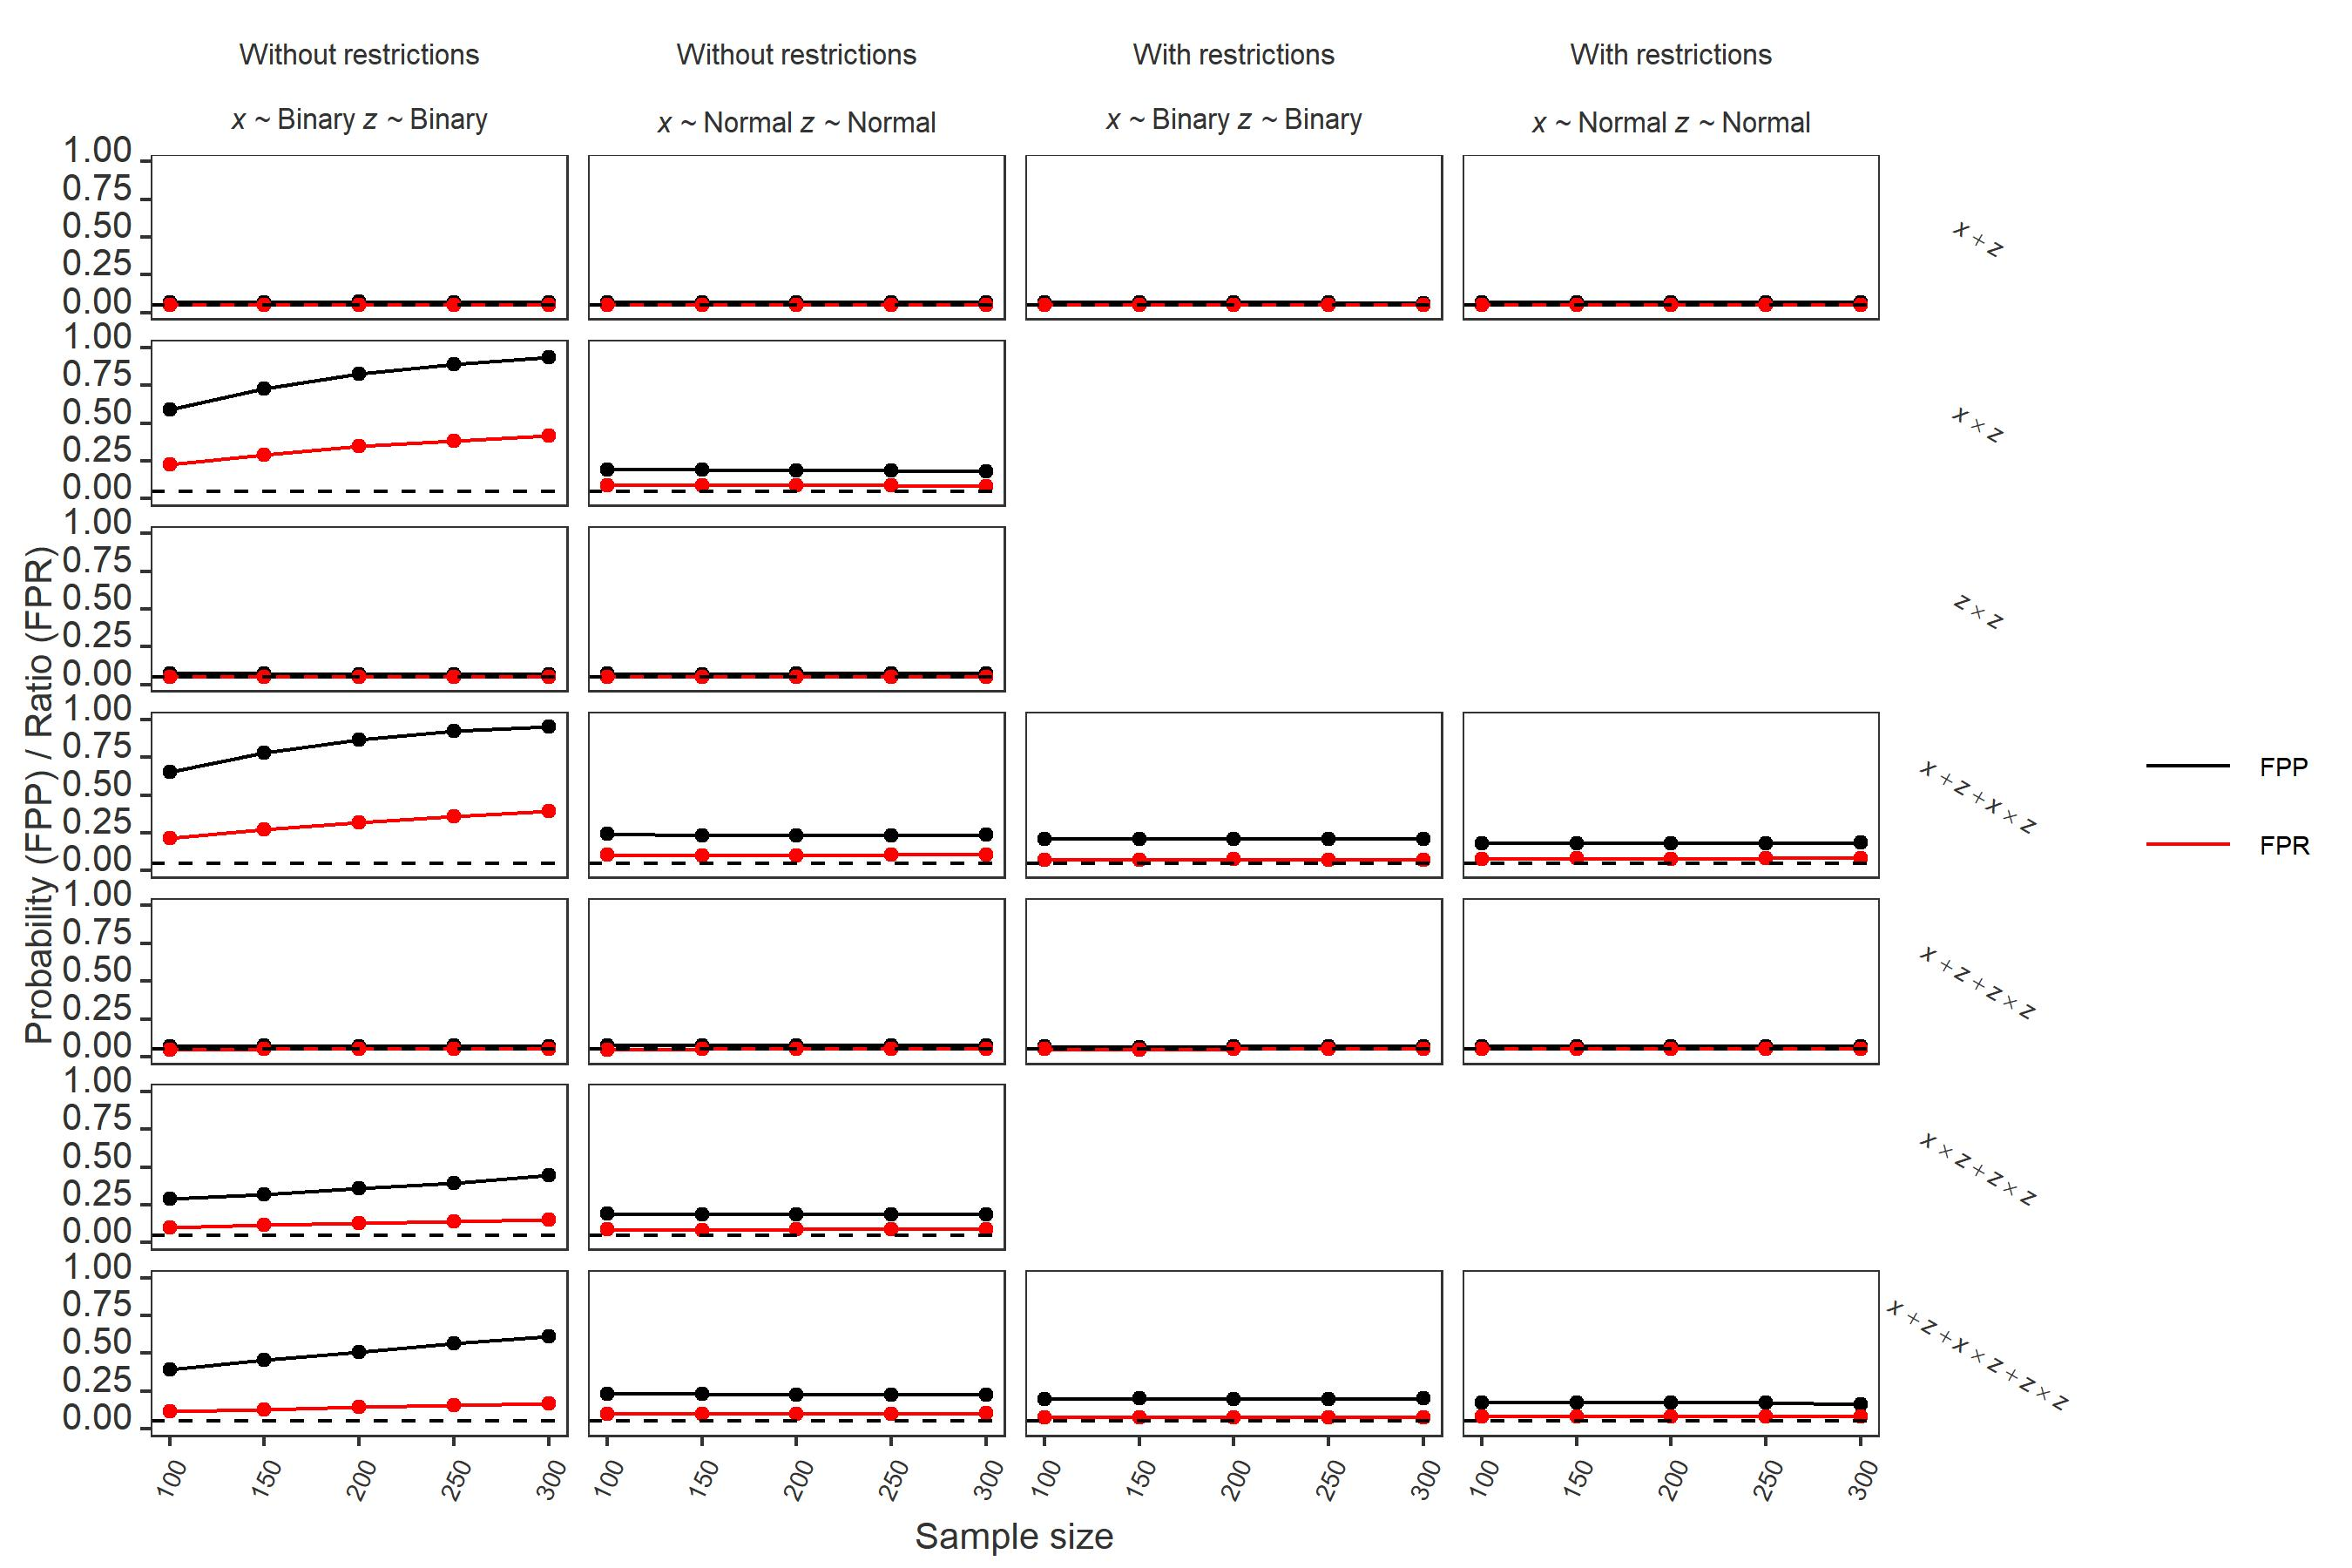
\includegraphics[width=0.9\textwidth]{R/Analysis/Result/Figures/Figure1D.jpeg}
\centering
\caption{The effect of increasing sample size on the false-positive probability and false-positive ratio. Black denotes the false-positive probability and red denotes the false-positive ratio. The description of the figure is otherwise the same as for Figure 1.}
\label{fig:mainfigure}
\end{figure}

\subsection{Correlation}
A higher correlation between the dependent variable and the covariates also influenced the rates of FPP and FPR for some model sets. In general, the FPP and FPR were higher as the correlation increased and main effects did not follow interactions. The model sets with the highest increase for both the FPP and FPR were the sets that contained HCI. The effect was most pronounced when the variable of interest and covariates were binary (as can be seen in Figure S2). The increase in the FPP for these sets was between 15\% and 23\% when the correlation increased from \textit{r}=0.2 to \textit{r}=0.3. When the correlation increased from \textit{r}=0.3 to \textit{r}=0.4, the FPP increased only for those sets where there was still room for an increase, since a high number of the sets already had the FPP close to 100\%. The increase in correlation also affected the FPR for the same sets increasing it to as high as 10\%. When main effects were present, the FPP and FPR were not as affected compared to when main effect were not present.